\documentclass[a4paper,10pt]{report}
\usepackage{cours}
\usepackage{pifont}

\begin{document}
\everymath{\displaystyle}

\begin{center}
\textit{{ {\huge TD 12 : Espaces vectoriels normés}}}
\end{center}


\bigskip

\noindent Dans la suite, $\mathbb{K}$ désignera $\mathbb{R}$ ou $\mathbb{C}$ et $n$, $p$ seront deux entiers naturels non nuls.

\medskip

\begin{center}
\textit{{ {\large Normes}}}
\end{center}

\medskip



\begin{Exercice}{} Pour tout $A = (a_{i,j})_{\substack{1 \leq i \leq n \\ 1 \leq j \leq p}} \in \mathcal{M}_{n,p}(\K)$, on pose :
$$\Vert A \Vert_{1}  = \sum_{i = 1}^{n} \sum_{j = 1}^{p} \vert a_{i,j} \vert, \; \Vert A \Vert_{\infty}  = \max_{1 \leq i \leq n,1 \leq j \leq p} \vert a_{i,j} \vert $$
Montrer que $A \mapsto \Vert A \Vert_{1}$ et $A \mapsto \Vert A \Vert_{\infty}$ définissent des normes sur $\mathcal{M}_{n,p}(\K)$.
\end{Exercice}

%\corr 
%
%\noindent $\rhd$ Montrons que $A \mapsto \Vert A \Vert_{1}$ définit une norme sur $\mathcal{M}_{n,p}(\K)$.
%
%\begin{itemize}
%\item Pour tout $A \in \mathcal{M}_{n,p}(\K)$, $\Vert A \Vert_{1} \geq 0$.
%\item Prouvons l'homogénéité. Soient $\lambda \in \mathbb{K}$ et $A=(a_i{i,j}) \in \mathcal{M}_{n,p}(\K)$. Alors :
%\begin{align*}
%\Vert \lambda A \Vert_1 & = \sum_{i = 1}^{n} \sum_{j = 1}^{p} \lambda \vert a_{i,j} \vert \\
%& = \sum_{i = 1}^{n} \sum_{j = 1}^{p} \vert \lambda \vert \, \vert a_{i,j} \vert \quad \hbox{(homogénéité du module)} \\
%& = \vert \lambda \vert  \sum_{i = 1}^{n} \sum_{j = 1}^{p} \vert \lambda \vert \, \vert a_{i,j} \vert  \quad \hbox{(linéarité)} \\
%& = \vert \lambda \vert \Vert A \Vert_1 
%\end{align*}
%\item Montrons la séparation. Soit $A=(a_{i,j}) \in \mathcal{M}_{n,p}(\mathbb{K})$ telle que $\Vert A \Vert_1=0$. Alors :
%$$ \sum_{i = 1}^{n} \sum_{j = 1}^{p} \vert \lambda \vert \, \vert a_{i,j} \vert =0$$
%Or, une somme de termes positifs est nulle si et seulement si tous les termes sont nuls donc :
%$$ \forall (i,j) \in \Interv{1}{n} \times \Interv{1}{p}, \; \vert a_{i,j} \vert =0$$
%et ainsi :
%$$  \forall (i,j) \in \Interv{1}{n} \times \Interv{1}{p}, \;  a_{i,j}  =0$$
%La matrice $A$ est donc la matrice nulle. Réciproquement, la matrice nulle a une norme nulle.
%\item Montrons l'inégalité triangulaire. Soient $A=(a_{i,j})$ et $B=(b_{i,j})$ deux matrices de $\mathcal{M}_{n,p}(\mathbb{K})$. Alors :
%\begin{align*}
%\Vert A+B \Vert_1 & =  \sum_{i = 1}^{n} \sum_{j = 1}^{p} \vert \lambda \vert \, \vert a_{i,j} +b_{i,j} \vert  \\
%& \leq \sum_{i = 1}^{n} \sum_{j = 1}^{p} \vert \lambda \vert \, \vert a_{i,j} \vert + \vert b_{i,j} \vert \quad \hbox{(inégalité triangulaire du module)}  \\
%& = \sum_{i = 1}^{n} \sum_{j = 1}^{p} \vert \lambda \vert \, \vert a_{i,j} \vert  + \sum_{i = 1}^{n} \sum_{j = 1}^{p} \vert \lambda \vert \,  \vert b_{i,j} \vert\vert \quad \hbox{(linéarité)} \\
%& = \Vert A \Vert_1 + \Vert B \Vert_1 
%\end{align*}
%\end{itemize}
%Ainsi, $A \mapsto \Vert A \Vert_1$ est une norme sur $\mathcal{M}_{n,p}(\mathbb{K})$.
%
%\medskip
%
%\noindent $\rhd$ Montrons que $A \mapsto \Vert A \Vert_{\infty}$ définit une norme sur $\mathcal{M}_{n,p}(\K)$.
%
%\begin{itemize}
%\item Pour tout $A \in \mathcal{M}_{n,p}(\K)$, $\Vert A \Vert_{\infty} \geq 0$.
%\item Prouvons l'homogénéité. Soient $\lambda \in \mathbb{K}$ et $A=(a_{i,j}) \in \mathcal{M}_{n,p}(\K)$. Pour tout $(i,j) \i,n (i,j) \in \Interv{1}{n} \times \Interv{1}{p}$,
%$$ \vert \lambda a_{i,j} \vert = \vert \lambda \vert \vert a_{i,j}\vert \leq \vert \lambda \vert \Vert A \Vert_{\infty}$$
%On en déduit que :
%$$ \Vert \lambda A \Vert_{\infty} \leq \vert \lambda \vert \Vert A \Vert_{\infty}$$
%Si $\lambda = 0$, l'égalité est évidente. Si $\lambda \neq 0$, on applique l'inégalité précédente avec $\dfrac{1}{\lambda}$ au lieu de $\lambda$ et $\lambda A$ au lieu de $A$ ce qui donne :
%$$ \Vert  A \Vert_{\infty} \leq \left\vert \dfrac{1}{\lambda} \right\vert \Vert \lambda A \Vert_{\infty}$$
%ou encore :
%$$ \vert \lambda \vert \Vert A \Vert_{\infty} \leq \Vert \lambda A \Vert_{\infty}$$
%et on obtient ainsi l'inégalité (par double inégalité).
%
%
%\item Montrons la séparation. Soit $A=(a_{i,j}) \in \mathcal{M}_{n,p}(\mathbb{K})$ telle que $\Vert A \Vert_{\infty}=0$. Pour tout $(i,j) \i,n (i,j) \in \Interv{1}{n} \times \Interv{1}{p}$,
%$$ 0 \leq \vert a_{i,j} \vert \leq \Vert A \Vert_{\infty}=0$$
%donc :
%$$ \forall (i,j) \in \Interv{1}{n} \times \Interv{1}{p}, \; \vert a_{i,j} \vert =0$$
%et ainsi :
%$$  \forall (i,j) \in \Interv{1}{n} \times \Interv{1}{p}, \;  a_{i,j}  =0$$
%La matrice $A$ est donc la matrice nulle. Réciproquement, la matrice nulle a une norme nulle.
%\item Montrons l'inégalité triangulaire. Soient $A=(a_{i,j})$ et $B=(b_{i,j})$ deux matrices de $\mathcal{M}_{n,p}(\mathbb{K})$. Alors pour tout $(i,j) \i,n (i,j) \in \Interv{1}{n} \times \Interv{1}{p}$, d'après l'inégalité triangulaire liée au module :
%$$ \vert a_{i,j} + b_{i,j} \vert \leq \vert a_{i,j} \vert + \vert b_{i,j} \vert \leq \Vert A \Vert_{\infty} + \Vert B \Vert_{\infty}$$
%et ainsi :
%$$ \Vert A+B \Vert_{\infty}  \leq \Vert A \Vert_{\infty} + \Vert B \Vert_{\infty}$$
%\end{itemize}
%Ainsi, $A \mapsto \Vert A \Vert_{\infty}$ est une norme sur $\mathcal{M}_{n,p}(\mathbb{K})$.




\begin{Exercice}{} Pour tout $(x,y) \in \mathbb{R}^2$, on pose :
$$ N((x,y)) = \sup_{t \in [0,1]} \vert x+ty \vert$$

\begin{enumerate}
\item Montrer que la fonction $N$ est bien définie et que c'est une norme sur $\mathbb{R}^2$.
\item Tracer la boule unité ouverte de $\mathbb{R}^2$ pour cette norme.
\end{enumerate}
\end{Exercice}

%\corr 
%
%\begin{enumerate}
%\item Soit $(x,y) \in \mathbb{R}^3$. La fonction $t \mapsto \vert x+ty \vert$ est continue sur le segment $[0,1]$ donc bornée et admet un maximum sur ce segment. Ainsi, $N((x,y))$ est bien défini.
%
%\medskip
%
%\noindent Montrons que $N$ est une norme sur $\mathbb{R}^2$. Pour gagner en efficacité, remarquons que :
%$$ N((x,y)) = \Vert f_{x,y} \Vert_{\infty}$$
%où $f_{x,y} : t \mapsto x+ty$ et $\Vert \cdot \Vert_{\infty}$ est la norme infini sur $[0,1]$.
%
%\begin{itemize}
%\item Pour tout $(x,y) \in \mathbb{R}^2$, $N((x,y)) \geq 0$.
%\item Montrons l'homogénéité. Soient $\lambda \in \mathbb{R}$ et $(x,y) \in \mathbb{R}^2$. Alors :
%\begin{align*}
%N(\lambda (x,y)) & = \Vert f_{\lambda x, \lambda y} \Vert_{\infty} \\
%& = \Vert \lambda f_{x,y} \Vert_{\infty} \\
%& = \vert \lambda \vert \Vert \lambda f_{x,y} \Vert_{\infty} \quad \hbox{(par homogénéité)} \\
%& = \vert \lambda \vert N((x,y)) 
%\end{align*}
%\item Montrons la séparation. Soit $(x,y) \in \mathbb{R}^2$ tel que $N((x,y))=0$. Alors pour tout $t \in [0,1]$,
%$$ 0 \leq \vert x+ty \vert \leq \sup_{t \in [0,1]} \vert x+ty \vert = N((x,y))=0 $$
%On en déduit que $x+ty=0$. Pour $t=0$, on obtient $x=0$ puis pour $t=1$, on obtient $y=0$. Finalement, $(x,y)=(0,0)$. Réciproquement, le couple nul a une norme nulle.
%\item Montrons l'inégalité triangulaire. Soient $(x,y)$ et $(x',y')$ deux couples de $\mathbb{R}^2$. Alors :
%\begin{align*}
%N((x,y)+(x',y')) & = N((x+x',y+y')) \\
%& = \Vert f_{x+x',y+y'} \Vert_{\infty} \\
%& = \Vert f_{x,y} + f_{x',y'} \Vert_{\infty} \\
%& \leq \Vert f_{x,y} \Vert + \Vert f_{x',y'} \Vert_{\infty} \quad \hbox{(inégalité triangulaire)} \\
%& = N((x,y))+ N((x',y')) 
%\end{align*}
%\end{itemize}
%Ainsi, $N$ est une norme sur $\mathbb{R}^2$.
%\item Soit $(x,y) \in \mathbb{R}^2$. La fonction $f_{x,y}$ est une fonction monotone donc la valeur maximale en valeur absolue est atteinte en $0$ ou en $1$ donc :
%$$ N((x,y)) = \max \lbrace \vert x+ 0 \times y \vert, \vert x+ 1 \times y \vert \rbrace = \max \lbrace \vert x \vert, \vert x+y \vert \rbrace$$
%On en déduit que :
%\begin{align*}
%(x,y) \in B((0,0),1) & \Longleftrightarrow \max \lbrace \vert x \vert, \vert x+y \vert \rbrace <1 \\
%& \Longleftrightarrow \vert x \vert < 1 \; \hbox{ et } \; \vert x+y \vert < 1 \\
%& \Longleftrightarrow -1 <x<1 \; \hbox{ et } \;  -1 < x+y<1 \\
%& \Longleftrightarrow - 1<x<1 \; \hbox{ et } \; -1-x <y <1-x
%\end{align*}
%Voici une représentation graphique :
%
%\medskip
%
%\begin{center}
%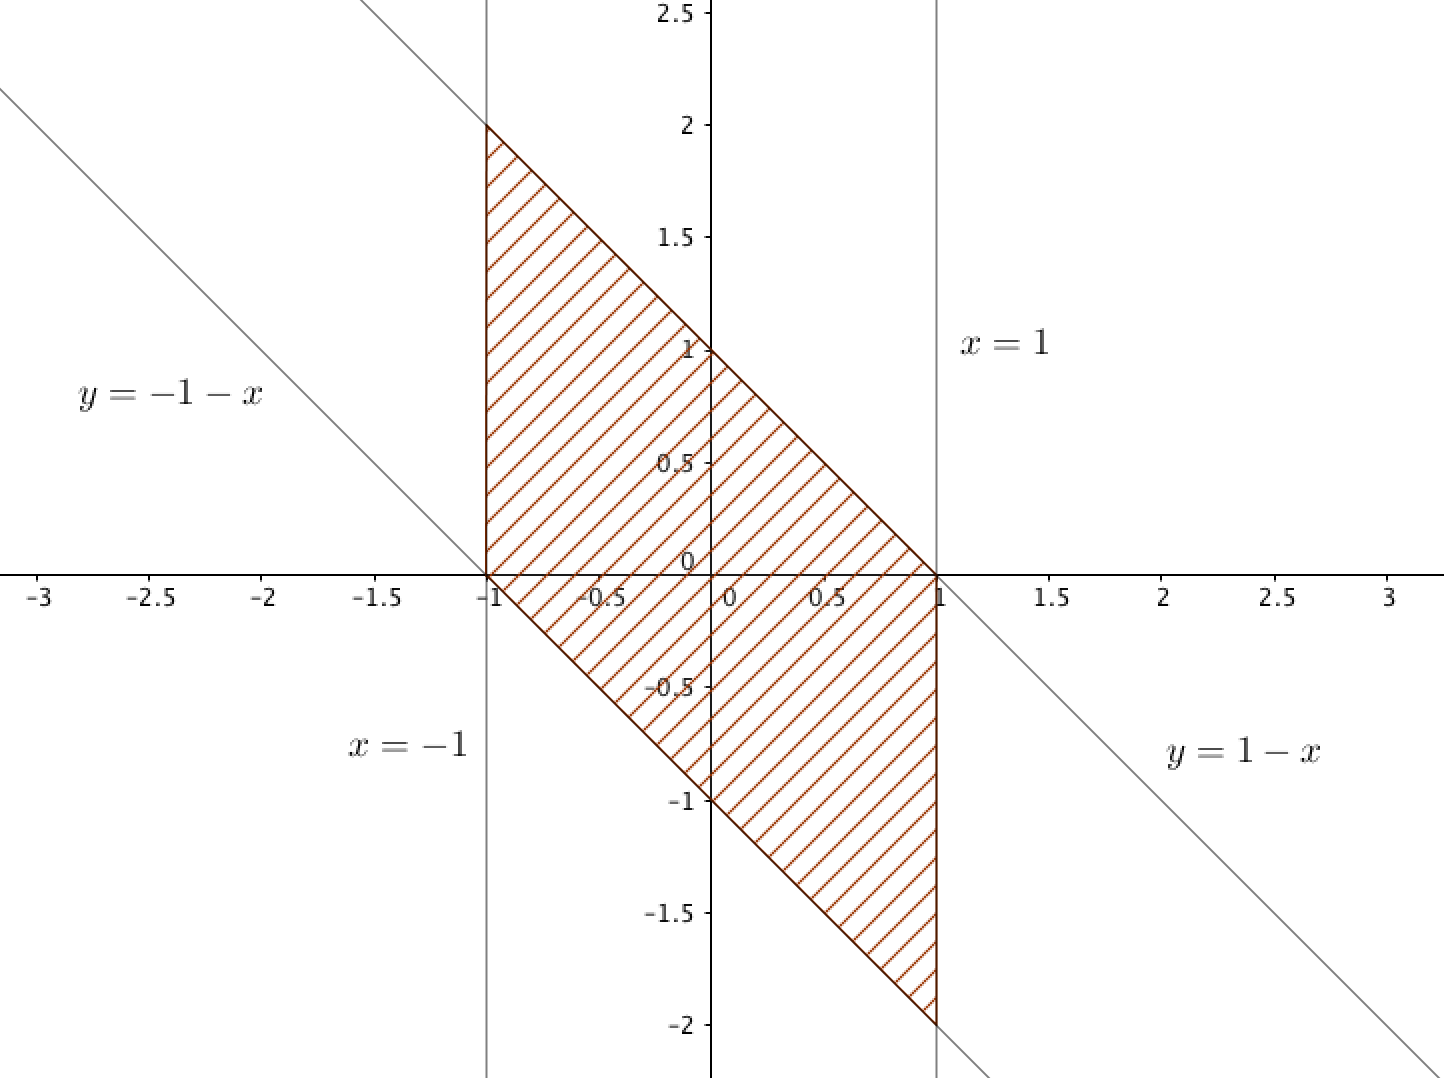
\includegraphics[scale=0.4]{BouleU}
%\end{center}
%\end{enumerate}

\begin{Exercice}{} Pour tout $P  \in \R_n[X ]$, on pose :
$$N(P) = \sum_{k = 0}^{ n } \vert P^{(k)} (0) \vert $$
Montrer que $N$ définit une norme sur $\R_n [X]$.
\end{Exercice}

%\corr $N$ est une application de $\R_n[X ]$ dans $\mathbb{R}_+$.
%
%\begin{itemize}
%\item Montrons l'homogénéité. Soient $\lambda \in \mathbb{R}$ et $P \in  \R_n[X ]$. Alors :
%\begin{align*}
%N(\lambda P) & =  \sum_{k = 0}^{ n } \vert (\lambda P)^{(k)} (0) \vert  \\
%& =  \sum_{k = 0}^{ n }  \vert \lambda P^{(k)} (0) \vert \quad \hbox{(linéarité de la dérivation)} \\
%& =  \sum_{k = 0}^{ n } \vert \lambda \vert \vert P^{(k)} (0) \vert \\
%& = \vert \lambda \vert \sum_{k = 0}^{ n } \vert P^{(k)} (0) \vert \\
%& = \vert \lambda \vert N(P) 
%\end{align*}
%\item Montrons la séparation. Soit $P \in  \R_n[X ]$ tel que $N(P)=0$. Alors :  
%$$ \sum_{k = 0}^{ n } \vert P^{(k)} (0) \vert =0$$
%Une somme de termes positifs est nulle si et seulement si tous les termes sont nuls. Ainsi, pour tout entier $k \in \Interv{0}{n}$,
%$$  \vert P^{(k)} (0) \vert = 0$$
%et donc 
%$$   P^{(k)} (0)  = 0$$
%Or $P$ a un degré au plus égal à $n$ donc d'après la formule de Taylor :
%$$ P(X) = \sum_{k=0}^n \dfrac{P^{k}(0)}{k!} X^k = 0$$
%Ainsi, $P$ est nul. Réciproquement, si $P$ est nul alors $N(P)=0$.
%\item Montrons l'inégalité triangulaire. Soient $P$ et $Q$ deux polynômes de $\mathbb{R}_n[X]$. Alors :
%\begin{align*}
%N(P+Q) & = \sum_{k = 0}^{ n } \vert (P+Q)^{(k)} (0) \vert \\
%& = \sum_{k = 0}^{ n } \vert P^{(k)} (0) +  Q^{(k)} (0) \vert \quad \hbox{(linéarité de la dérivation)} \\
%& \leq \sum_{k = 0}^{ n } \vert P^{(k)} (0) \vert +  \vert Q^{(k)} (0) \vert \quad \hbox{(inégalité triangulaire)} \\
%& = \sum_{k = 0}^{ n } \vert P^{(k)} (0) \vert + \sum_{k = 0}^{ n } \vert P^{(k)} (0) \vert \\
%& = N(P) + N(Q)
%\end{align*}
%Ainsi, $N$ définit une norme sur $\mathbb{R}_n[X]$.
%\end{itemize}


\begin{Exercice}{} Pour tout $A = (a_{i,j})_{1 \leq i,j \leq n} \in \mathcal{M}_{n}(\mathbb{C})$, on pose :
  \[
  \Vert A \Vert = \max_{1 \leq i \leq n} \sum_{j = 1}^{n}  \vert a_{i,j} \vert
  \]
  \begin{enumerate}
  \item Montrer que $A \mapsto \Vert A \Vert$ définit une norme sur $\mathcal{M}_{n}(\mathbb{C})$.
  \item Montrer cette norme est une \textit{norme d'algèbre}, c'est-à-dire vérifiant :
    \[
    \forall A,B \in \mathcal{M}_{n}(\mathbb{C}),  \; \Vert AB \Vert \leq \Vert A \Vert \, \Vert B \Vert
    \]
  \end{enumerate}
\end{Exercice}

%\corr 
%
%\begin{enumerate}
%\item Pour tout $A \in \mathcal{M}_n(\mathbb{C})$, $\Vert A \Vert$ est bien défini car c'est le maximum d'un ensemble fini non vide.
%
%\begin{itemize}
%\item Pour tout $A \in \mathcal{M}_n(\mathbb{C})$, $\Vert A \Vert \geq 0$.
%\item Montrons l'homogénéité. Soient $\lambda \in \mathbb{C}$ et $A=(a_{i,j}) \in \mathcal{M}_n(\mathbb{C})$. Pour tout $i \in \Interv{1}{n}$,
%\begin{align*}
% \sum_{j=1}^n \vert \lambda a_{i,j} \vert & =  \sum_{j=1}^n \vert \lambda \vert \vert a_{i,j} \vert \\
% & =  \vert \lambda \vert \sum_{j=1}^n \vert a_{i,j} \vert \\
% & \leq \vert \lambda \vert \Vert A \Vert
% \end{align*}
% et ainsi :
% $$ \Vert \lambda A \Vert \leq \vert \lambda \vert \Vert A \Vert$$
% Si $\lambda=0$, l'égalité est évidente. Si $\lambda \neq 0$, on applique l'inégalité précédente avec $\dfrac{1}{\lambda}$ au lieu de $\lambda$ et $\lambda A$ au lieu de $A$ :
% $$ \Vert A \Vert \leq \dfrac{1}{\vert \lambda \vert} \Vert \lambda A \Vert$$
% et ainsi :
% $$  \vert \lambda \vert \Vert A \Vert \leq \Vert \lambda A \Vert$$
% ce qui donne l'égalité (par double inégalité).
% \item Montrons la séparation. Soit $A \in \mathcal{M}_n(\mathbb{C})$ tel que $\Vert A \Vert =0$. Alors pour tout $i \in \Interv{1}{n}$,
%$$ 0 \leq \sum_{j=1}^n \vert a_{i,j} \vert \leq \Vert A \Vert = 0$$
%donc :
%$$ \sum_{j=1}^n \vert a_{i,j} \vert$$
%Une somme de termes positifs est nulle si et seulement si tous les termes sont nuls donc finalement pour tout $(i,j) \in \Interv{1}{n}^2$,
%$$  \vert a_{i,j} \vert = 0$$
%et ainsi :
%$$ a_{i,j}=0$$
%Ainsi, $A$ est nulle. Réciproquement, si $A$ est nulle, $\Vert A \Vert$ est nul.
%\item Montrons l'inégalité triangulaire. Soient $A=(a_{i,j})$ et $B=(b_{i,j})$, deux matrices de $\mathcal{M}_n(\mathbb{C})$. On a :
%$$ \Vert A+B \Vert = \max_{1 \leq i \leq n} \sum_{j=1}^n \vert a_{i,j}+ b_{i,j} \vert$$
%Soit $i \in \Interv{1}{n}$. Alors d'après l'inégalité triangulaire (liée au module) :
%\begin{align*}
% \sum_{j=1}^n \vert a_{i,j}+ b_{i,j} \vert &  \leq \sum_{j=1}^n \vert a_{i,j} \vert + \vert b_{i,j} \vert \\
% & = \sum_{j=1}^n \vert a_{i,j} \vert + \sum_{j=1}^n \vert b_{i,j} \vert  \\
% & \leq \Vert A \Vert + \Vert B \Vert
% \end{align*}
%Ainsi,
%$$ \Vert A+B \Vert \leq \Vert A \Vert + \Vert B \Vert$$
%\end{itemize}
%Ainsi, $A \mapsto \Vert A \Vert$ définit une norme sur $\mathcal{M}_{n}(\mathbb{C})$.
%\item Soient $A=(a_{i,j})$ et $B=(b_{i,j})$, deux matrices de $\mathcal{M}_n(\mathbb{C})$. Alors :
%$$ \Vert AB \Vert = \max_{1 \leq i \leq n} \sum_{j=1}^n \vert (AB)_{i,j} \vert$$
%Soit $i \in \Interv{1}{n}$. Alors :
%\begin{align*}
%\sum_{j=1}^n \vert (AB)_{i,j} \vert & = \sum_{j=1}^n \left\vert \sum_{k=1}^n a_{i,k} b_{k,j} \right\vert \\
%& \leq  \sum_{j=1}^n  \sum_{k=1}^n \vert a_{i,k} \vert \vert b_{k,j} vert \quad \hbox{(inégalité triangulaire)} \\
%& = \sum_{k=1}^n  \sum_{j=1}^n \vert a_{i,k} \vert \vert b_{k,j} \vert  \\
%& =  \sum_{k=1}^n \vert a_{i,k} \vert  \sum_{j=1}^n \vert b_{k,j} \vert  
%\end{align*}
%Or on a pour tout $k \in \Interv{1}{n}$,
%$$ \sum_{j=1}^n \vert b_{k,j} vert   \leq \Vert B \Vert$$
%On en déduit que :
%\begin{align*}
%\sum_{j=1}^n \vert (AB)_{i,j} \vert  \leq  \sum_{k=1}^n \vert a_{i,k} \vert \Vert B \Vert \\
%& = \Vert B \Vert  \sum_{k=1}^n \vert a_{i,k} \vert \\
%& \leq \Vert B \Vert \Vert A \Vert
%\end{align*}
%Cette inégalité est vérifiée pour tout $i \in \Interv{1}{n}$ donc :
%$$ \Vert AB \Vert \leq \Vert B \Vert \Vert A \Vert$$
%\end{enumerate}





\medskip

\begin{center}
\textit{{ {\large Comparaisons de normes, normes équivalentes}}}
\end{center}

\medskip

\begin{Exercice}{} On considère deux normes définies sur $E= \mathcal{C}([0,1], \mathbb{R})$ de la manière suivante :
$$ \forall f \in E, \; \Vert f \Vert_1 = \int_0^1 \vert f(t) \vert \dt \; \hbox{ et } \; \Vert f \Vert_{\infty} = \max_{x \in [0,1]} \vert f(x) \vert$$
\begin{enumerate}
\item Pour tout entier $n \geq 1$, on définit la fonction $f_n : [0,1] \rightarrow \mathbb{R}$ par :
$$ \forall x \in [0,1], \; f_n(x) = \left\lbrace \begin{array}{cl}
-n^2x+n & \hbox{ si } x \in [0,1/n] \\
0 & \hbox{ sinon}
\end{array}\right.$$
Représenter graphiquement les fonctions $f_1$, $f_2$ et $f_3$.
\item Montrer que les normes $1$ et infini ne sont pas équivalentes sur $E$.
\end{enumerate}
\end{Exercice}

\begin{Exercice}{\ding{80}}
\begin{enumerate}
\item Montrer que $N$, définie par :
$$ N(f) = \sup_{[0,1]} \vert f''+2f'+f \vert $$
est une norme sur $E = \lbrace f \in \mathcal{C}^2([0,1]) \, \vert \, f(0)=f'(0)=0 \rbrace \cdot$
\item Soient $f \in E$ et $h$ définie pour tout $t \in [0,1]$ par $h(t)=f(t)e^t$. Montrer que pour tout $t \in [0,1]$,
$$ h(t) = \int_{0}^t (t-u) h''(u) \textrm{d}u$$
\item Montrer qu'il existe $a \in \mathbb{R}_+^{*}$ tel que pour tout $f \in E$,
$$ \Vert f \Vert_{\infty} \leq a N(f)$$
\item Minimiser $a$.
\end{enumerate}
\end{Exercice}

%\corr 
%\begin{enumerate}
%\item Soit $f \in E$. Alors $f$ est de classe $\mathcal{C}^2$ sur $[0,1]$ donc $f''+2f'+f$ est continue sur le segment $[0,1]$ et donc bornée sur celui-ci. Ainsi $N(f)$ existe. L'application $N$ est donc bien définie.
%
%\medskip
%
%\noindent Remarquons que pour tout $f \in E$,
%$$ N(f) = \Vert f''+2f"+f \Vert_{\infty}$$
%En utilisant que la norme infini est une norme sur $E$, toutes les propriétés à vérifier sont immédiates sauf la séparation. Soit $f \in E$ tel que $N(f)=0$. En utilisant que la norme infini est une norme sur $E$, on en déduit que $f''+2f"+f=0$ et en particulier $f$ est solution de l'équation différentielle linéaire homogène d'ordre deux suivante :
%$$ y''+ 2y'+y = 0$$
%Sachant que $f(0)=f'(0)=0$ et que la fonction nulle est aussi solution de cette équation différentielle et vérifie les mêmes conditions (nulle en $0$ et dérivée nulle en $0$), on en déduit d'après le théorème de Cauchy-Lipschitz que $f$ est nulle par unicité.
%
%\item La fonction $f$ est $\mathcal{C}^2$ sur $[0,1]$ donc $h$ aussi. On a pour tout $t \in [0,1]$,
%$$ h'(t) = f'(t)e^t +f(t)e^t \quad \hbox{ et } \quad h''(t) =(f''(t)+2f'(t)+f(t))e^t$$
%Posons pour tout $t \in [0,1]$,
%$$ g(t) = \int_{0}^t (t-u) h''(u) \textrm{d}u = t \int_{0}^t h''(u) \textrm{d}u - \int_{0}^t u h''(u) \textrm{d}u$$
%$g$ est bien définie car $h''$ est continue sur $[0,1]$. En utilisant le théorème fondamental de l'analyse, on a pour tout $t \in [0,1]$,
%$$ g'(t) = \int_{0}^t h''(u) \textrm{d}u + th''(t)- th''(t) = \int_{0}^t h''(u) \textrm{d}u$$
%et en le réutilisant :
%$$ g''(t) = h''(t)$$
%Ainsi $g''$ et $h''$ coïncident sur l'intervalle $[0,1]$ donc il existe une constante $C$ tel que pour tout $t \in [0,1]$,
%$$ g'(t)=h'(t) + C$$
%Or $g'(0)=h'(0)=0$ (car $f$ appartient à $E$) donc $g'$ et $h'$ coïncident sur l'intervalle $[0,1]$ donc il existe une constante $K$ tel que pour tout $t \in [0,1]$,
%$$ g(t)=h(t)+K$$
%Or $g(0)=h(0)=0$ donc finalement $g=h$.
%\item Soient $f \in E$ et $h$ définies comme précédemment. Alors pour tout $t \in [0,1]$,
%$$ f(t) = e^{-t} \int_{0}^t (t-u) h''(u) \textrm{d}u$$
%ce qui implique (sachant que les bornes sont dans le bon sens et que $t-u \geq 0$ si $u \in [0,t]$) :
%$$  \vert f(t) \vert \leq e^{-t} \int_{0}^t (t-u) \vert h''(u) \vert  \textrm{d}u$$
%Or on a :
%$$ \vert h''(u) \vert = \vert f''(u)+2f'(u)+f(u)) \vert e^u \leq N(f) e^u$$
%et ainsi :
%$$ \vert f(t) \vert \leq  N(f) e^{-t} \int_{0}^t (t-u) e^u\textrm{d}u$$
%En remarquant que :
%$$ \int_{0}^t (t-u) e^u\textrm{d}u = t \int_{0}^t e^u \textrm{d}u - \int_{0}^t u e^u \textrm{d}u$$
%et en utilisant une intégration par parties, on a :
%$$  e^{-t} \int_{0}^t (t-u) e^u\textrm{d}u = e^{-t}(e^t-t-1) = 1 -(t+1)e^{-t}$$
%Posons $m : t \mapsto 1-(t+1)e^{-t}$. Alors $m' : t \mapsto t e^{-t}$ donc $m$ est croissante sur $[0,1]$ et son maximum vaut $m(1)= 1-2e^{-1}$. Finalement, pour tout $t \in [0,1]$,
%$$ \vert f(t) \vert \leq (1-2e^{-1}) N(f) $$
%Ainsi, $a = 1-2e^{-1} \in \mathbb{R}_+^{*}$ convient.
%\item Reprenons la fonction $m$ précédente. On a $m(0)=m'(0)=1$ donc $m$ appartient à $E$. On a $m'' : t \mapsto (1-t)e^{-t}$ donc pour tout $t \in [0,1]$,
%$$ m''(t)+2m'(t)+m(t) = (1-t)e^{-t} +2t e^{-t} +1 -(t+1)e^{-t} = 1$$
%Donc $N(m) =1$ et on a déjà montré que $\Vert m \Vert_{\infty}=1-2 e^{-1}$ donc :
%$$ \Vert m \Vert_{\infty}=(1-2 e^{-1}) N(m)$$
%La valeur $a = 1-2e^{-1}$ est donc minimale.
%\end{enumerate}

\medskip

\begin{center}
\textit{{ {\large Ouverts, fermés, bornés}}}
\end{center}

\medskip



\begin{Exercice}{} Les parties $A$ suivantes sont-elles bornées dans $E$ ?

\begin{enumerate}
\item $A= \lbrace (x,y,z)\in (\R_+)^3 \, \vert \,  \ x+y+z\leq 1\rbrace$ et $E= \mathbb{R}^3$.
\item $A = \lbrace (x,y)\in\R^2 \, \vert \, x^2=y(y-1) \rbrace$ et $E= \mathbb{R}^2$.
\item $A = \lbrace (x,y)\in\R^2 \, \vert \, x^2+xy+y^2\leq1 \rbrace$ et $E= \mathbb{R}^2$.
\item L'ensemble $A$ des matrices à coefficients dans $\lbrace -1,1 \rbrace$ et $E = \mathcal{M}_n(\mathbb{R})$.
\end{enumerate}
\end{Exercice}

%\begin{enumerate}
%\item Utilisons la norme $1$. Pour tout $(x,y,z) \in A$, on a :
%\begin{align*}
%\Vert (x,y,z) \Vert_1 & = \vert x \vert + \vert y \vert + \vert z \vert \\
%& = x+y+z \quad \hbox{ car } (x,y,z) \in  (\R_+)^3 \\
%&  \leq 1
%\end{align*}
%Ainsi, $A$ est borné.
%\item Pour tout entier $n \geq 1$, $ n(n-1) \geq 0$. Posons alors :
%$$ x_n = \sqrt{n(n-1)}$$
%On a alors :
%$$ x_n^2= n(n-1)$$
%et ainsi $(x_n,n) \in A$. Utilisons la norme infini. Pour tout entier $n \geq 1$,
%$$ \Vert (x_n,n) \Vert_{\infty} = \max(x_n,n) \geq n \underset{n \rightarrow + \infty}{\longrightarrow} + \infty$$
%Ainsi, $A$ n'est pas borné.
%\item Soit $(x,y) \in A$. Alors :
%\begin{align*}
%x^2+xy+y^2 & = \left( x+\dfrac{y}{2}  \right)^2 - \dfrac{y^2}{4}+ y^2 \\
%& = \left( x+\dfrac{y}{2}  \right)^2  + \dfrac{3y^2}{4} \\
%& \leq 1
%\end{align*}
%Les deux termes étant positifs, on en déduit que :
%$$ \left( x+\dfrac{y}{2}  \right)^2 \leq 1 \; \hbox{ et } \; \dfrac{3y^2}{4} \leq 1 $$
%La deuxième inégalité est équivalent à :
%$$ y^2 \leq \dfrac{4}{3}$$
%ou encore :
%$$ - \dfrac{2}{\sqrt{3}} \leq y \leq \dfrac{2}{\sqrt{3}}$$
%La première inégalité est alors équivalente à :
%$$ -1 \leq x+\dfrac{y}{2} \leq 1 $$
%ou encore :
%$$ -1 - \dfrac{y}{2} \leq x \leq 1- \dfrac{y}{2}$$
%et finalement à :
%$$ -1 - \dfrac{2}{\sqrt{3}} \leq x \leq 1 + \dfrac{2}{\sqrt{3}}$$
%On en déduit que :
%\begin{align*}
%\Vert (x,y) \Vert_1 & = \vert x \vert + \vert y \vert \\
%& \leq 1+ \dfrac{2}{\sqrt{3}} + \dfrac{2}{\sqrt{3}} \\
%& = 1 + \dfrac{4}{\sqrt{3}}
%\end{align*}
%Ainsi, $A$ est borné.
%\item Utilisons la norme infini de $\mathcal{M}_n(\mathbb{R})$. Pour tout $M \in A$,
%$$ \Vert M \Vert_{\infty} = \max_{1 \leq i,j \leq n} \vert a_{i,j} \vert  \leq 1$$
%Ainsi, $A$ est borné.
%\end{enumerate}

\begin{Exercice}{} Repr\'esenter graphiquement les ensembles suivants. Sont-ils des ouverts ? Des ferm\'es ? Des parties bornées ?
\begin{enumerate}
\item $A = \lbrace (x,y)\in\R^2 \, \vert \, x^2 < 1 \hbox{ et } y> 1\rbrace$
\item $B = \lbrace (x,y)\in\R^2 \, \vert \, x^2 < 1 \hbox{ et } y \geq 1\rbrace$
%\item $C = \lbrace (x,y)\in\R^2 \, \vert \, x+2y^2=1\rbrace$
%\item $D = \lbrace (x,y)\in\R^2 \, \vert \, x^2 -2x  + y^2+6y \leq -6\rbrace$
\end{enumerate}
\end{Exercice}

%\corr
%
%\begin{enumerate}
%\item Voici une représentation graphique : 
%
%\begin{center}
%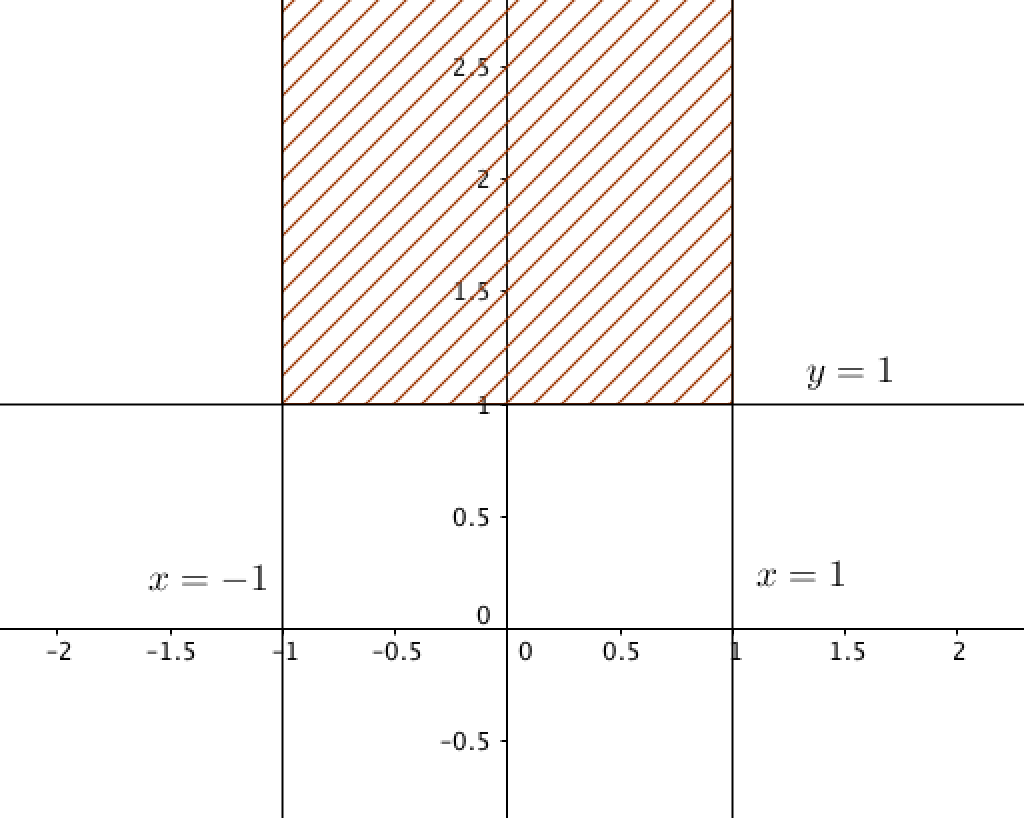
\includegraphics[scale=0.5]{im1}
%\end{center}
%\begin{itemize}
%\item Montrons que $A$ est un ouvert de $\mathbb{R}^2$. Soit $(x_0,y_0) \in A$. Alors :
%$$ -1 < x_0 < 1 \; \hbox{ et } \; y_0>1$$
%Posons :
%$$ r = \min \left( \dfrac{1-\vert x_0\vert}{2}, \dfrac{y_0-1}{2} \right)$$
%Utilisons la norme infini. Pour tout $(x,y) \in B((x_0,y_0),r)$, on a :
%$$ \Vert (x,y)-(x_0,y_0) \Vert_{\infty} <r $$
%Ainsi :
%$$ \max (\vert x-x_0 \vert, \vert y-y_0 \vert)<r$$
%On en déduit que :
%$$ \vert x-x_0 \vert < r \leq \dfrac{1-\vert x_0\vert}{2}$$
%et ainsi d'après l'inégalité triangulaire :
%\begin{align*}
%\vert x \vert & \leq \vert x-x_0 \vert + \vert x_0 \vert \\
%& <\dfrac{1-\vert x_0\vert}{2} + + \vert x_0 \vert \\ 
%& < \dfrac{\vert x_0 \vert + 1 }{2}\\
%& < 1
%\end{align*}
%car $\vert x_0 \vert <1$. On sait aussi que :
%$$  \vert y-y_0 \vert < r \leq \dfrac{y_0-1}{2}$$
%Ainsi, 
%\begin{align*}
%y-1 &= y-y_0 + y_0-1 \\
%& \geq - \vert y- y_0 \vert + y_0-1 \\
%& > - \dfrac{y_0-1}{2} + y_0-1 \\
%& = \dfrac{y_0-1}{2}\\
%& >0
%\end{align*}
%car $y_0>1$. On en déduit que $(x,y) \in B((x_0,y_0),r)$. Ainsi, $A$ est un ouvert de $\mathbb{R}^2$.
%\item $A$ est n'est pas un fermé car pour tout entier $n \geq 1$,
%$$ \left(0,1+ \dfrac{1}{n} \right) \in A$$
%mais :
%$$ \lim_{n \rightarrow + \infty} \left(0,1 + \dfrac{1}{n}\right) = (0,1) \notin A$$
%\item $A$ n'est pas un ensemble borné de $\mathbb{R}^2$ car pour tout entier $n \geq 2$,
%$$ (0,n) \in A$$
%et 
%$$ \Vert (0,n) \Vert_1 = n \underset{n \rightarrow + \infty}{\longrightarrow} + \infty$$
%\end{itemize}
%\item La représentation graphique est la même que celle de la question précédente. 
%\begin{itemize}
%\item L'ensemble $A$ n'est pas un ouvert car :
%$$ (0,1) \in A$$
%et 
%$$ \lim_{\varepsilon \rightarrow 0} (0,1- \varepsilon) = (0,1)$$
%alors que pour tout $\varepsilon>0$, $(0,1- \varepsilon) \notin A$. 
%\item L'ensemble $A$ n'est pas un fermé car  pour tout entier $n \geq 1$,
%$$ \left(1- \dfrac{1}{n},1\right) \in A$$
%mais :
%$$ \lim_{n \rightarrow + \infty} \left(1- \dfrac{1}{n},1\right) = (1,1) \notin A$$
%\item L'ensemble $A$ n'est pas borné (même preuve que dans la question précédente).
%\end{itemize}
%\end{enumerate}

\begin{Exercice}{} Montrer que $\left\{P\in\R_n[X], \, \dis\int_0^1P(t)dt= 1\right\}$ est un fermé.
\end{Exercice}

%\corr Soit $F$ cet ensemble. Remarquons que :
%$$ F = \lbrace P \in \mathbb{R}_n[X] \, \vert \, f(P)=0 \rbrace$$
%où $f: \mathbb{R}_n[X] \rightarrow \mathbb{R}$ est définie par :
%$$ f(P)= \int_0^1P(t)dt-1$$
%L'application $f$ est continue comme différence d'une forme linéaire sur un espace vectoriel de dimension finie (donc continue) et d'une application constante. Ainsi, $F$ est un fermé de $\mathbb{R}_n[X]$.

\begin{Exercice}{} Montrer que $\{M\in{\cal M}_n(\R) \, \vert \,  ^tM=-M\}$ est un fermé.
\end{Exercice}

%\corr Soit $F$ cet ensemble. Soit $(M_k)_{k \geq 0}$ une suite d'éléments de $F$ convergeant vers une matrice $M$ de $\mathcal{M}_n(\mathbb{R})$ :
%$$ \lim_{k \rightarrow + \infty} M_k = M$$
%Par convergence composante par composante, on a pour tout $(i,j) \in \Interv{1}{n}^2$,
%$$  \lim_{k \rightarrow + \infty} (M_k)_{i,j} = M_{i,j}$$
%Pour tout entier $k \geq 0$, $^t(M_k)=-M_k$ donc pour tout $(i,j) \in \Interv{1}{n}^2$,
%$$ (M_k)_{j,i} = - (M_k)_{i,j}$$
%Par passage à la limite, on en déduit que :
%$$ M_{j,i}=-M_{i,j}$$
%et ainsi, $^t M=-M$ donc $M \in F$. Finalement, $F$ est un fermé de $\mathcal{M}_n(\mathbb{R})$.

\begin{Exercice}{} L'ensemble $GL_n(\mathbb{R})$ est-il un fermé de $\mathcal{M}_n(\mathbb{R})$?
\end{Exercice} 

%\corr Non car :
%$$ \lim_{k \rightarrow + \infty} \dfrac{1}{k} I_n = 0_n$$
%On a donc une suite d'éléments de $GL_n(\mathbb{R})$ convergeant vers une matrice n'appartenant pas à $GL_n(\mathbb{R})$.


\begin{Exercice}{} Soit $A$ et $B$ deux parties d'un espace vectoriel normé telles que $A \subset B$. Montrer que $\mathring{A} \subset \mathring{B}$ et $\overline{A} \subset \overline{B}$.
\end{Exercice}

%\corr Soit $x \in \mathring{A}$. Il existe un réel strictement positif $r>0$ tel que :
%$$ B(a,r) \subset A \subset B$$
%donc $a \in  \mathring{B}$. Ainsi, $\mathring{A} \subset \mathring{B}$.
%
%\medskip
%
%\noindent Soit $x \in \overline{A}$. Il existe une suite d'éléments de $A$ (donc de $B$ car $A \subset B$) convergeant vers $x$. Donc $x \in \overline{B}$.


\begin{Exercice}{\ding{80}} Soit $F$ un sous-espace vectoriel d'un espace vectoriel normé $E$, distinct de $E$. Montrer que $F$ est d'intérieur vide.
\end{Exercice}

%\corr Supposons par l'absurde que $F$ n'est pas d'intérieur vide. Il existe donc un vecteur $a$ de $E$ et un réel strictement positif $r>0$ tel que :
%$$ B_f(a,r) \subset F$$
%Soit $x \in E$ tel que $\Vert x \Vert <r$. On a :
%$$ \Vert a-(a+x) \Vert =  \Vert -x \Vert = \Vert x \Vert < r$$
%donc $a+x$ appartient à $B_f(a,r)$ donc appartient à $F$. Or $F$ est un sous-espace vectoriel de $E$ donc :
%$$ x = (a+x) -a \in F$$
%car $a+x$ et $a$ appartiennent à $F$. Soit $y$ un vecteur quelconque de $E$. Alors par homogénéité :
%$$ \left\Vert \dfrac{r}{2} \times \dfrac{y}{\Vert y \Vert } \right\Vert  = \dfrac{r}{2} \dfrac{\Vert y \Vert }{\Vert y \Vert } = \dfrac{r}{2} < r$$
%Ainsi :
%$$ \dfrac{r}{2} \times \dfrac{y}{\Vert y \Vert } \in F$$
%Or $F$ est un sous-espace vectoriel de $E$ donc tout multiple de ce vecteur appartient à $F$ donc $y$ appartient à $F$. On en déduit que $E \subset F$ et sachant que $F \subset E$, on a $E=F$ ce qui est absurde.

\begin{Exercice}{} Soit $SL_n(\mathbb{R})$ l'ensemble des matrices de $\mathcal{M}_n(\mathbb{R})$ de déterminant égal à $1$.
\begin{enumerate}
\item Montrer que $SL_n(\mathbb{R})$ est un fermé de $\mathcal{M}_n(\mathbb{R})$.
\item Montrer que $SL_n(\mathbb{R})$ est d'intérieur vide.
\end{enumerate}
\end{Exercice}

%\corr 
%
%\begin{enumerate}
%\item Soit $(A_k)_{k \geq 0}$ une suite d'éléments de $SL_n(\mathbb{R})$ convergeant vers une matrice $A \in \mathcal{M}_n(\mathbb{R})$. Montrons que $A$ appartient à $SL_n(\mathbb{R})$. L'application $\textrm{det} : \mathcal{M}_n(\mathbb{R}) \rightarrow \mathbb{R}$ est continue car le déterminant est une forme linéaire sur $\mathcal{M}_n(\mathbb{R})$ donc sachant que  :
%$$ \lim_{k \rightarrow + \infty} A_k = A$$
%on a :
%$$ \lim_{k \rightarrow + \infty} \textrm{det}(A_k) = \textrm{det}(A)$$
%Or pour tout entier $k \geq 0$, $A_k$ appartient à $SL_n(\mathbb{R})$ donc $\textrm{det}(A_k)=1$ et ainsi $\textrm{det}(A)=1$ donc $A$ appartient à $SL_n(\mathbb{R})$. Finalement, $SL_n(\mathbb{R})$ est un fermé de $\mathcal{M}_n(\mathbb{R})$.
%\item Par l'absurde, supposons que $SL_n(\mathbb{R})$ n'est pas d'intérieur vide. Il existe donc une matrice $A \in SL_n(\mathbb{R})$ et un réel strictement positif $r>0$ tel que :
%$$ B(A,r) \subset SL_n(\mathbb{R})$$
%Remarquons maintenant que :
%$$ \lim_{\varepsilon \rightarrow 0} (1+ \varepsilon) A= A$$
%donc pour $\varepsilon>0$ assez petit, $(1+ \varepsilon) A \in B(a,r)$ et ainsi $(1+ \varepsilon) A \in SL_n(\mathbb{R})$ ce qui est absurde car par multilinéarité : 
%$$ \textrm{det}((1+ \varepsilon)A)= (1+\varepsilon)^n \textrm{det}(A) = (1+\varepsilon)^n \neq 1$$
%Ainsi, $SL_n(\mathbb{R})$ est d'intérieur vide.
%\end{enumerate}

\begin{Exercice}{} Soit $\mathcal{D}$ l'ensemble des matrices diagonalisables de $\mathcal{M}_2(\mathbb{R})$. L'ensemble $\mathcal{D}$ est-il un fermé de $\mathcal{M}_2(\mathbb{R})$? Un ouvert de $\mathcal{M}_2(\mathbb{R})$?
\end{Exercice}

%\corr On a :
%$$ \lim_{n \rightarrow + \infty} \begin{pmatrix}
%1+ \dfrac{1}{n} & 1 \\
%0 & 1- \dfrac{1}{n} \\
%\end{pmatrix} = \begin{pmatrix}
%1 & 1 \\
%0 & 1 \\
%\end{pmatrix}$$
%Chaque matrice $\begin{pmatrix}
%1+ \dfrac{1}{n} & 1 \\
%0 & 1- \dfrac{1}{n} \\
%\end{pmatrix}$ est diagonalisable car elle admet deux valeurs propres distinctes mais $\begin{pmatrix}
%1 & 1 \\
%0 & 1 \\
%\end{pmatrix}$ n'est pas diagonalisable car cette matrice admet pour unique valeur propre $1$ : si elle était diagonalisable, elle serait semblable à $I_2$ donc égale à $I_2$ ce qui est faux. Ainsi, $\mathcal{D}$ n'est pas un fermé de $\mathcal{M}_2(\mathbb{R})$.
%
%\medskip
%
%\noindent On a : 
%$$ \lim_{\varepsilon \rightarrow 0} \begin{pmatrix}
%0 & \varepsilon \\
%0 & 0 
%\end{pmatrix} = 0_2$$
%La matrice $0_2$ est diagonalisable. Si $\mathcal{D}$ était un ouvert de $\mathcal{M}_2(\mathbb{R})$, dans un voisinage de $0_2$, toutes les matrices seraient diagonalisables. C'est faux car $\begin{pmatrix}
%0 & \varepsilon \\
%0 & 0 
%\end{pmatrix}$ tend vers $0_2$ quand $\varepsilon$ tend vers $0$ et chacune de ces matrices n'est pas diagonalisable car cette matrice admet pour unique valeur propre $0$ : si elle était diagonalisable, elle serait semblable à $0_2$ donc égale à $0_2$ ce qui est faux. Ainsi, $\mathcal{D}$ n'est pas un ouvert de $\mathcal{M}_2(\mathbb{R})$.


\begin{Exercice}{\ding{80}} Soit $E= \mathcal{M}_n(\mathbb{R})$. On note $\mathcal{N}$ l'ensemble des matrices nilpotentes de $E$.

\begin{enumerate}
\item Montrer que si $A$ est une matrice nilpotente de $E$ alors $A^n=0_n$.
\item Montrer que $\mathcal{N}$ est un fermé de $E$.
\item 
\begin{enumerate}
\item Soient $A \in \mathcal{N}$, $\alpha \in \mathbb{R}^*$ et $M=I_n+ \alpha A$. Montrer que $\textrm{det}(M)=1$.
\item En déduire que toute boule ouverte de centre $A$ contient une matrice inversible puis que $\mathcal{N}$ est d'intérieur vide.
\end{enumerate}
\end{enumerate}
\end{Exercice}
%
%\corr 
%
%\begin{enumerate}
%\item $A$ est nilpotente donc il existe un entier $k \geq 1$ tel que $A^k=0_n$. Le polynôme $X^k$ est donc un polynôme annulateur de $A$ : les valeurs propres de $A$ sont donc racines de ce polynôme. Ainsi, $A$ admet uniquement $0$ comme valeur propre. Le polynôme caractéristique de $A$ étant unitaire et de degré $n$, on en déduit que :
%$$ \chi_A(X)=X^n$$
%D'après le théorème de Cayley-Hamilton, on en déduit que :
%$$ A^n=0_n$$
%\item Soient $(A_k)_{k \geq 0}$ une suite d'éléments de $\mathcal{N}$ convergeant vers une matrice $A$ de $E$ :
%$$ \lim_{k \rightarrow + \infty} A_k = A$$
%D'après la question précédente, pour tout entier $k \geq 0$, $A_k^n=0_n$. Or l'application $f : E \rightarrow E$ définie par $f(M)=M^n$ est continue sur $E$ (chaque composante de $f(M)$ est polynômiale en les coefficients de $M$). On en déduit que :
%$$ \lim_{k \rightarrow + \infty} f(A_k) = f(A)$$
%ou encore :
%$$ \lim_{k \rightarrow + \infty} A_k^n = A^n$$
%et ainsi, $A^n=0_n$ donc $A$ est nilpotente donc appartient à $\mathcal{N}$. Ainsi, $\mathcal{N}$ est un fermé de $E$.
%\item
%
%\begin{enumerate}
%\item La matrice $A$ est nilpotente donc $A^n=0_n$ et ainsi :
%$$( \alpha A)^n = \alpha^n A^n = 0_n$$
%donc $\alpha A$ est aussi nilpotente. Son polynôme caractéristique est $X^n$ qui est scindé sur $\mathbb{R}$ donc $\alpha A$ est trigonalisable et $\alpha A$ est donc semblable à une matrice triangulaire supérieure $T$ dont tous les coefficients diagonaux sont $0$ (car $0$ est la seule valeur propre de $\alpha A$). Il existe une matrice inversible $P$ tel que :
%$$ \alpha A = P TP^{-1}$$
%et ainsi :
%$$ I_n+ \alpha A = I_n + PTP^{-1} = PP^{-1}+ PTP^{-1} = P(I_n+ T)P^{-1}$$
%Ainsi, $I_n+ \alpha A$ et $P(I_n+ T)P^{-1}$ sont semblables donc :
%$$ \textrm{det}(I_n+ \alpha A) = \textrm{det}(I_n+ T)=1$$
%car $I_n+T$ est une matrice triangulaire supérieure avec des coefficients diagonaux égaux à $1$.
%Ainsi, $\textrm{det}(M)=1$.
%\item Soit $A$ une matrice appartenant à $\mathcal{N}$. Soit $B$ une boule ouverte de centre $A$. On a :
%$$ \lim_{\varepsilon \rightarrow 0} A+ \varepsilon I_n = A$$
%donc pour $\varepsilon>0$ assez petit, $A+ \varepsilon I_n$ appartient à $B$. Or on a :
%$$ \textrm{det}(A+ \varepsilon I_n) = \textrm{det}(\varepsilon((1/\varepsilon)A+  I_n)) = \varepsilon^n \textrm{det}(\varepsilon((1/\varepsilon)A+  I_n))$$
%par multilinéarité du déterminant et donc d'après la question précédente,
%$$ \textrm{det}(A+ \varepsilon I_n)  = \varepsilon^n \neq 0$$
%Ainsi, $A+ \varepsilon I_n$ est inversible et répond donc à la question.
%
%\medskip
%
%\noindent Montrons que $\mathcal{N}$ est d'intérieur vide. Si par l'absurde $\mathcal{N}$ n'était pas d'intérieur vide, il existerait une matrice $A \in \mathcal{N}$ et une boule ouverte $B$ de rayon $r>0$ centrée en $A$ telle que $B \subset N$. D'après la question précédente, il existe une matrice $P$ inversible appartenant à $B$ et donc à $\mathcal{N}$. C'est absurde car une matrice inversible ne peut pas être nilpotente (une matrice nilpotence admet $0$ pour valeur propre). Ainsi, par l'absurde, on a montré que $\mathcal{N}$ était d'intérieur vide.
%\end{enumerate}
%\end{enumerate}


\begin{Exercice}{} On dit qu'une matrice carrée est \textit{stochastique} si ses coefficients appartiennent à $[0,1]$ et que la somme de chaque ligne vaut $1$. Montrer que l'ensemble $\mathcal{S}$, constitué des matrices stochastiques de $\mathcal{M}_n(\mathbb{R})$, est un convexe compact de $\mathcal{M}_n(\mathbb{R})$.
\end{Exercice} 

%\corr Procédons en trois étapes.
%
%\medskip
%
%\noindent $\rhd$ Montrons que $\mathcal{S}$ est convexe, c'est-à-dire :
%$$ \forall (A,B) \in \mathcal{S}^2, \; \forall \lambda \in [0,1], \; \lambda A+(1-\lambda)B \in \mathcal{S}$$
%Soient $(A,B) \in \mathcal{S}^2$ et $\lambda \in [0,1]$. En notant $A=(a_{i,j})$ et $B=(b_{i,j})$, on a :
%$$ \lambda A+ (1- \lambda) B = (\lambda a_{i,j} + (1- \lambda) b_{i,j})$$
%Tous les coefficients $a_{i,j}$ et$ b_{i,j}$ sont appartiennent à $[0,1]$ qui est convexe donc les réels $\lambda a_{i,j} + (1- \lambda) b_{i,j}$ aussi. Par définition de $\mathcal{S}$, on sait que pour tout $i \in \Interv{1}{n}$,
%$$ \sum_{j=1}^n a_{i,j} = \sum_{j=1}^n b_{i,j} = 1$$
%et ainsi :
%\begin{align*}
%\sum_{j=1}^n \lambda a_{i,j} + (1 - \lambda) b_{i,j} & = \lambda   \sum_{j=1}^n a_{i,j} + (1 - \lambda)  \sum_{j=1}^n b_{i,j}  \\
%& = \lambda + 1- \lambda \\
%& = 1
%\end{align*}
%Ainsi, $\lambda A+ (1- \lambda)B$ appartient à $\mathcal{S}$. Finalement, $\mathcal{S}$ est convexe.
%
%\medskip
%
%\noindent Montrons que $S$ est un fermé de $\mathcal{M}_n(\mathbb{R})$. Soit $(A_k)_{k \geq 0}$ une suite d'éléments de $S$ convergeant vers $A=(a_{i,j}) \in \mathcal{M}_n(\mathbb{R})$. Montrons que $A$ appartient à $\mathcal{S}$. Notons pour tout $k \geq 0$, $A_k = (a_{i,j}^k)$. Par convergence composante par composante, on a pour tout $(i,j) \in \Interv{1}{n}^2$,
%$$ \lim_{k \rightarrow + \infty} a_{i,j}^k = a_{i,j}$$
%Or les matrices $A_k$ appartiennent à $\mathcal{S}$ donc tous les coefficients $a_{i,j}^k$ appartient à $[0,1]$ donc par passage à la limite, $a_{i,j} \in [0,1]$. De, pour tout entier $k \geq 0$ et tout entier $i \in \Interv{1}{n}$,
%$$ \sum_{p=1}^n a_{i,p}^k = 1$$
%Donc par passage à la limite quand $k$ tend vers $+ \infty$ :
%$$ \sum_{p=1}^n a_{i,p} = 1$$
%On en déduit que $A$ appartient à $\mathcal{S}$. Ainsi, $\mathcal{S}$ est fermé.
%
%\medskip
%
%\noindent $\rhd$ Utilisons la norme $1$ définie dans un autre exercice. Pour toute matrice $A=(a_{i,j})$ de $\mathcal{M}_n(\mathbb{R})$,
%\begin{align*}
%\Vert A \Vert_1 & = \sum_{i = 1}^{n} \sum_{j = 1}^{n} \vert a_{i,j} \vert \\
%& = \sum_{i = 1}^{n} \sum_{j = 1}^{n}  a_{i,j}  \\
% & = \sum_{i = 1}^{n} 1 \\
% & = n
%\end{align*}
%Ainsi, $\mathcal{S}$ est inclus dans la sphère de centre la matrice nulle et de rayon $n$ donc $\mathcal{S}$ est bornée.
\medskip

\begin{center}
\textit{{ {\large Fonctions à valeurs réelles}}}
\end{center}

\medskip



\begin{Exercice}{} Étudier la continuité de $f : \mathbb{R}^2 \rightarrow \mathbb{R}$ définie par $ f((x,y))=  \max(x,y)$.
\end{Exercice}

%\corr Soit $(x,y) \in \mathbb{R}^2$. On sait que :
%$$ \max(x,y)+ \min(x,y) = x+y$$
%et 
%$$ \max(x,y)-\min(x,y) = \vert x-y \vert$$
%On en déduit que :
%$$ f(x,y)= \max(x,y) = \dfrac{x+y+ \vert x-y \vert}{2}$$
%Les fonctions polynômiales (en les composantes) sont bornées sur $\mathbb{R}^3$ et la valeur absolue l'est sur $\mathbb{R}$ donc par composition, $f$ est continue sur $\mathbb{R}^2$.

\begin{Exercice}{} Étudier la continuité de $f : \mathbb{R}^2 \rightarrow \mathbb{R}$ définie par $f((x,y))= \ln(1 + \sqrt{x^2+y^2})$.
\end{Exercice}

%\corr La fonction $(x,y) \mapsto x^2+y^2$ est polynômiale (en les composantes) donc continue sur $\mathbb{R}^2$ et à valeurs positives, $t \mapsto \sqrt{t}$ est continue sur $\mathbb{R}_+$ et à valeurs positives donc :
%$$ (x,y) \mapsto 1+ \sqrt{x^2+y^2}$$
%est continue et strictement positive sur $\mathbb{R}^2$. La fonction $\ln$ est continue sur $\mathbb{R}_+^{*}$ donc $f$ est continue sur $\mathbb{R}^2$.

\begin{Exercice}{} Étudier la continuité de la fonction $f : \mathbb{R}^2 \rightarrow \mathbb{R}$ définie par :
$$ f((x,y)) = \left\lbrace \begin{array}{cl}
\dfrac{x^4 y}{x^6+y^4} & \hbox{ si } (x,y) \neq (0,0) \\
0 & \hbox{ si } (x,y)=(0,0) \\
\end{array}\right.$$
\end{Exercice}

%\corr La fonction $f$ est continue en tout point $(x,y) \neq (0,0)$ par quotient de fonctions polynômiales et sachant que dans ce cas, $x^6+y^4 \neq 0$. 
%
%\medskip
%
%\noindent Étudions la continuité de $f$ en $(0,0)$. Celle-ci est continue en $(0,0)$ si :
%$$ \lim_{(x,y) \rightarrow (0,0)} f((x,y)) =f((0,0))= 0$$
%Pour tout réel $x$ non nul,
%$$ f((x,x^2)) = \dfrac{x^6}{x^6+x^8} = \dfrac{1}{1+x^2}$$
%Si $x$ tend vers $0$, $(x,x^2)$ tend vers $(0,0)$ et pourtant :
%$$ \lim_{x \rightarrow 0} \dfrac{1}{1+x^2} = 1 \neq 0$$
%donc $f$ n'est pas continue en $(0,0)$.

\begin{Exercice}{} Étudier la continuité en $(0,0)$ de la fonction $f : \R^{2} \rightarrow \R$ définie par :
  \[
  f((x,y)) =
  \begin{cases}
    \frac{xy}{\vert x \vert + \vert y \vert} & \hbox{ si } (x,y) \neq (0,0) \\
    \, \; 0 & \hbox{ si } (x,y)=(0,0)
  \end{cases}
  \]
\end{Exercice}

%\corr La fonction $f$ est continue en $(0,0)$ si :
%$$ \lim_{(x,y) \rightarrow (0,0)} f((x,y)) =f((0,0))= 0$$
%Utilisons la norme $1$. Pour tout couple non nul $(x,y)$, on a :
%\begin{align*}
%0 \leq \vert f((x,y)) \vert & = \dfrac{\vert x \vert \times \vert y \vert}{\vert x \vert + \vert y \vert} \\
%& \leq \dfrac{(\vert x \vert + \vert y \vert)(\vert x \vert + \vert y \vert)}{\vert x \vert + \vert y \vert} \\
%& = \vert x \vert + \vert y \vert \\
%& = \Vert (x,y) \Vert_1
%\end{align*}
%Ainsi, si $(x,y)$ tend vers $(0,0)$, on en déduit par théorème d'encadrement que :
%$$  \lim_{(x,y) \rightarrow (0,0)} f((x,y)) =f((0,0))= 0$$
%et donc $f$ est continue en $(0,0)$.




\begin{Exercice}{} Montrer que $\dis \max \left\lbrace x^5y^5 e^{z-2} \, \vert \, (x,y,z) \in (\mathbb{R}_+)^3 \hbox{ vérifiant } x+y+z =1 \right\rbrace$ existe.
\end{Exercice}

%\corr La fonction $(x,y,z) \mapsto x^5y^5 e^{z-2}$ est continue sur $\mathbb{R}^3$ (par produit de fonctions qui le sont). Il suffit de montrer que :
%$$K= \lbrace (x,y,z) \in \in (\mathbb{R}_+)^3 \, \vert \, x+y+z=1 \rbrace$$
%est un compact de $\mathbb{R}^3$ (c'est-à-dire : un ensemble fermé borné).
%
%\begin{itemize}
%\item Soit $((x_n,y_n,z_n))_{n \geq 0}$ une suite d'éléments de $K$ convergeant vers $(a,b,c) \in \mathbb{R}^3$. Montrons que $(a,b,c) \in K$. Pour tout entier $n \geq 0$, $x_n$, $y_n$ et $z_n$ sont des réels positifs donc par stabilité par inégalité large, $a$, $b$ et $c$ aussi. Pour tout entier $n \geq 0$,
%$$ x_n + y_n + z_n = 1$$
%Par passage à la limite, on en déduit que :
%$$ a+b+c=1$$
%Ainsi, $(a,b,c) \in K$. L'ensemble $K$ est donc fermé.
%\item Montrons que $K$ est borné. Utilisons la norme $1$. Pour tout $(x,y,z) \in K$,
%\begin{align*}
%\Vert (x,y,z) \Vert_1 & = \vert x \vert + \vert y \vert + \vert z \vert \\
%& = x+y+z \quad \hbox{ car } (x,y,z) \in \mathbb{R}_+^{3} \\
%& = 1
%\end{align*}
%Ainsi, $K$ est inclus dans la sphère unité donc est borné.
%\end{itemize}
%L'ensemble $K$ est compact donc $\dis \max \left\lbrace x^5y^5 e^{z-2} \, \vert \, (x,y,z) \in (\mathbb{R}_+)^3 \hbox{ vérifiant } x+y+z =1 \right\rbrace$ existe.
\newpage

\begin{center}
\textit{{ {\large Fonctions lipschitziennes}}}
\end{center}

\medskip


\begin{Exercice}{} Soit $I$ un intervalle de $\mathbb{R}$.

\begin{enumerate}
\item Soient $(k,k') \in (\mathbb{R}_+)^2$ et $(\alpha, \beta) \in \mathbb{R}^2$. Montrer que si $f : I \rightarrow \mathbb{R}$ est $k$-lipschitzienne et si $g : I \rightarrow \mathbb{R}$ est $k'$-lipschitzienne alors $\alpha f+ \beta g$ est $\vert \alpha \vert k  + \vert \beta \vert k'$-lipschitzienne.
\item Soit $f : I \rightarrow \mathbb{R}$ une fonction lipschitzienne de rapport $k \geq 0$. Montrer que les fonctions $f^+$ et $f^{-}$, définies pour tout $x \in I$ par 
$$ f^+(x)= \max(0,f(x)) \hbox{ et } f^{-}(x) = \max(-f(x),0) $$
sont aussi $k$-lipschitziennes.
\end{enumerate}
\end{Exercice}

%\corr 
%
%
%\begin{enumerate}
%\item Soit $(x,y) \in I^2$. Alors :
%\begin{align*}
%\vert (\alpha f(x)+ \beta g(x))-(\alpha f(y)+ \beta g(y)) \vert & = \vert \alpha (f(x)-f(y)) + \beta (g(x)-g(y)) \vert \\
%& \leq \vert \alpha (f(x)-f(y)) \vert + \vert \beta (g(x)-g(y)) \vert \quad \hbox{(inégalité triangulaire)} \\
%& = \vert \alpha \vert \vert f(x)-f(y) \vert + \vert \beta \vert \vert g(x)-g(y) \vert \quad \hbox{(homogénéité)} \\
%& \leq k \vert \alpha \vert  \vert x-y \vert + k' \vert \beta \vert \vert x-y \vert 
%\end{align*}
%car $f$ et $g$ sont respectivement $k$ et $k'$ lipschitziennes. On en déduit que :
%$$ \vert (\alpha f(x)+ \beta g(x))-(\alpha f(y)+ \beta g(y)) \vert \leq (k \vert \alpha \vert + k' \vert \beta \vert) \vert x-y \vert$$
%Ainsi, $\alpha f+ \beta g$ est $(k \vert \alpha \vert + k' \vert \beta \vert)$-lipschitzienne.
%\item On a :
%$$ f^{+} + f^{-} = \vert f \vert \; \hbox{ et } \; f^{+}-f^{-} = f$$
%ce qui implique que :
%$$ f^{+} = \dfrac{\vert f \vert+f}{2} \; \hbox{ et } \dfrac{\vert f \vert - f}{2}$$
%On a supposé que $f$ était $k$-lipschitzienne donc pour tout $(x,y) \in I^2$, d'après l'inégalité triangulaire \og inverse \fg :
%\begin{align*}
%\vert \vert f(x) \vert - \vert f(y) \vert \vert & \leq \vert f(x)-f(y) \vert  \\
%& \leq k \vert x-y \vert
%\end{align*}
%Ainsi, $\vert f \vert$ est $k$-lipschitzienne. D'après la question précédente, appliquée avec $\alpha$ et $\beta$ égaux à $\dfrac{1}{2}$, on en déduit que $f^{+}$ est lipschitzienne avec rapport :
%$$ \left\vert \dfrac{1}{2} \right\vert k + \left\vert \dfrac{1}{2} \right\vert k = k$$
%On obtient de même que $f^{-}$ est $k-$lipschitzienne.
%\end{enumerate}








\begin{Exercice}{\ding{80}} Soit $A$ une partie non vide d'un espace vectoriel normé $E$. Pour tout $x \in E$, on pose :
$$d(x,A) = \inf_{a \in A} \Vert x- a \Vert$$

\begin{enumerate}
\item Justifier que $d$ est bien définie.
\item Montrer que $d$ est $1$-lipschitzienne.
\item Déterminer un exemple pour lequel $d(x,A)=0$ avec $x \notin A$.
\item Montrer que $A$ est fermé dans $E$ si et seulement si :
$$ \forall x \in E, \quad d(x,A)=0 \Longleftrightarrow x \in A $$
\end{enumerate}
\end{Exercice}

%\begin{enumerate}
%\item Soit $x \in E$. L'ensemble :
%$$ \lbrace \Vert x- a \Vert \, \vert \, a \in A \rbrace$$
%est un sous-ensemble de $\mathbb{R}$, minorée par $0$ (une norme est positive) et non vide (car $A$ l'est) donc cet ensemble admet une borne inférieure et ainsi, $d(x,A)$ est bien défini donc $d$ est bien défini.
%\item Soit $(x,y) \in E^2$. Pour tout $a \in A$,
%$$ \Vert x-a \Vert = \Vert x-y+y-a \Vert \leq \Vert x-y \Vert + \Vert y-a \Vert$$
%Par définition de $d(x,A)$, on a donc :
%$$ d(x,A) \leq \Vert x-y \Vert + \Vert y-a \Vert$$
%donc :
%$$ d(x,A) - \Vert x-y \Vert \leq \Vert y-a \Vert$$
%Cette inégalité était vérifiée pour tout $a \in A$, on en déduit que :
%$$ d(x,A) - \Vert x-y \Vert \leq d(y,A)$$
%et ainsi :
%$$ d(x,A)-d(y,A) \leq \Vert x-y \Vert$$
%Par symétrie du rôle de $x$ et de $y$, on a aussi :
%$$  d(y,A)-d(x,A) \leq \Vert y-x \Vert = \Vert x-y \Vert$$
%et ainsi :
%$$ \vert d(x,A)-d(y,A) \vert \leq \Vert x-y \Vert$$
%Ainsi, $d$ est $1$-lipschitzienne.
%\item Soient $A= \mathbb{R}_+^{*}$. On a :
%$$ d(0,A) = \inf \lbrace \vert x \vert \, \vert \, x \in \mathbb{R}_+^* \rbrace = \inf \lbrace x \, \vert \, x \in \mathbb{R}_+^* \rbrace = 0$$
%Pourtant, $0$ n'appartient pas à $A$.
%\item 
%
%\begin{itemize}
%\item Supposons que $A$ est fermé. Montrons que :
%$$ \forall x \in E, \quad d(x,A)=0 \Longleftrightarrow x \in A $$
%Soit $x \in E$. Si $x \in A$, on a :
%$$ 0 \leq d(x,A) \leq \Vert x-x\Vert = 0$$
%donc $d(x,A)=0$.
%
%\medskip
%
%\noindent Supposons maintenant que $d(x,A)=0$. Alors :
%$$ \inf_{a \in A} \Vert x- a \Vert = 0$$
%Il existe donc une suite $(a_n)_{n \geq 0}$ d'éléments de $A$ tel que :
%$$ \lim_{n \rightarrow + \infty} \Vert x-a_n \Vert = 0$$
%donc 
%$$ \lim_{n \rightarrow + \infty} a_n = x$$
%or $A$ est un fermé donc $x\in A$.
%\item Supposons maintenant que :
%$$  \forall x \in E, \quad d(x,A)=0 \Longleftrightarrow x \in A $$
%Montrons que $A$ est un fermé de $E$. Soit $(a_n)_{n \geq 0}$ une suite d'éléments de $A$ convergeant vers $a \in E$. Par définition de $d(a,A)$, on a pour tout entier $n \geq 0$,
%$$0 \leq d(a,A) \leq \Vert a_n -a \Vert$$
%Or on sait que :
%$$ \lim_{n \rightarrow + \infty} \Vert a_n -a \Vert = 0$$
%D'après le théorème d'encadrement, on en déduit $d(a,A)=0$ et donc d'après l'hypothèse, $a \in A$. Ainsi, $A$ est un fermé de $E$.
%\end{itemize}
%\end{enumerate}



%
%% Centrale MP 242 2007
%
%\exo Pour tout $(x,y) \in \mathbb{R}^2$, on pose :
%$$ N((x,y)) = \sup_{t \in \mathbb{R}} \frac{\vert y+tx \vert}{1+t+t^2}$$
%Montrer que la fonction $N$ est bien définie et que c'est une norme sur $\mathbb{R}^2$.
%  




%\exo Fixons une norme $X\longmapsto \Vert X \Vert$ sur $\mathcal{M}_{n,1}(\R)$. On définit trois applications $N_1$, $N_2$ et $N_3$ de $\mathcal{M}_n(\R)$ dans $\mathbb{R}_+$ par :
%$$\forall A\in {\cal M}_n(\R),\qquad N_1(A)=\dis\sup_{X\in{\cal  M}_{n,1}(\R)\setminus\{0\}}\dis\frac{\|AX\|}{\|X\|},\quad N_2(A)=\dis\sup_{\|X\|\leq 1}\|AX\| \quad\hbox{et}\quad N_3(A)=\dis\sup_{\|X\|= 1}\|AX\|.$$
%
%\begin{enumerate}
%	\item Démontrer que $N_1=N_2=N_3$ et que ces applications définissent une norme sur $\mathcal{M}_n(\R)$. On note désormais $N$ cette norme.
%	
%	\item Montrer que pour toutes matrices $A,B\in {\cal M}_{n}(\R),$ on a $N(AB)\leq N(A)N(B).$
%	
%	\item Déterminer $N$ lorsque $\Vert  \cdot \Vert=\Vert \cdot \Vert_1$ et lorsque $\Vert  \cdot \Vert=\Vert  \cdot\Vert_{\infty}$ (on identifie $\mathbb{R}^n$ et $\mathcal{M}_{n,1}(\mathbb{R}))$.
%\end{enumerate}
%

%\medskip
%
%%\exo 
%%
%%\begin{enumerate}
%%\item Montrer que l'union de deux ouverts d'un espace vectoriel normé est un ouvert de celui-ci.
%%\item Montrer que $GL_n(\mathbb{R})$ est un ouvert de $\mathcal{M}_n(\mathbb{R})$.
%%%\item Montrer que l'adhérence de $GL_n(\mathbb{R})$ est  $\mathcal{M}_n(\mathbb{R})$.
%%\end{enumerate}

\end{document}